\documentclass{article}
\usepackage{KJN}
\usepackage{a4wide,changebar}
\usepackage[numbered,framed]{mcode}
\usepackage{dcolumn}

\title{BRISK-based Natural Landmark Localisation for Robocup}
\author{Daniel Mankowitz: S1128165}
\date{3/11/2011}

\begin{document}
\maketitle

\newpage
\begin{abstract}
This is the abstract
\end{abstract}

\section{Introduction}
\label{sec:introduction}

\subsection{Background}
\label{sec:background}

\section{General Feature Extraction Techniques}
\label{sec:genFeatureExtract}

\subsection{2DSURF}
\label{sec:2dsurf}
The SURF feature extraction algorithm is based on approximating the Hessian matrix at every point in an image. The determinant of the Hessian is then computed at each point and is referred to as the blob response. This computation is performed over a number of different scales in scale-space as well as in image space in order to find local maxima. A non-maximal suppression is then performed and the local maxima that exist after this stage will be defined as interest points. Each interest point is represented by a descriptor of length $64$. Interest points in different images are then matched based on the Euclidean distance between their respective feature vectors. The smaller the distance, the more certain the match becomes. 

\subsubsection{Integral Images}
\label{sec:integralImages}
One of the big advantages in SURF over SIFT \cite{Lowe2004} is its computational efficiency. One of the important tools that are utilised in order to create this advantage in computation is called the Integral Image \cite{Bay2008}. An integral image computes the integral image value, $I_{int}(x,y)$ for pixel location $(x,y)$  as a sum of all pixel intensities found to the left and below the current pixel location until the origin. This is presented in \eqnref{eqn:integralImage}. The variable $I(x,y)$ is the individual pixel intensity at location $(x,y)$. Thus the value of each pixel can be interpreted as the area of the rectangle formed from the current pixel to the image origin. It is assumed that the image origin is in the top left corner of the image. \\

\begin{equation}
I_{int}(x,y) = \sum_{i=0}^{i \leq x}\sum_{j=0}^{j \leq y}I(x,y)
\label{eqn:integralImage}
\end{equation}

By computing the integral image, it is possible to reduce the calculation of any upright rectangular image to four operations. This is very useful when computing box filter convolutions that will be described in the sections to follow.\\

\subsubsection{Detector}
\label{2dsurfdetect}
The SURF detector is based on computing the determinant of the Hessian matrix. The Hessian matrix is a matrix of second order partial derivatives and, when calculated for an intensity image,  $I(x,y)$, it is of the form shown in \eqnref{eqn:hessian}.\\

\begin{equation}
Hessian = \left[ \begin{array}{cc} \frac{\partial I}{\partial x^2} & \frac{\partial I}{\partial x^2}\\
					    \frac{\partial I}{\partial x^2} & \frac{\partial I}{\partial x^2}\end{array} \right]
\label{eqn:hessian}
\end{equation}

The Hessian matrix is computed in order to identify local maxima and minima in the image. This is achieved by first computing the determinant, also know as the discriminant, of the Hessian matrix. The determinant of the Hessian is shown in \eqnref{eqn:determinant}. If the determinant of the Hessian is negative then a local extrumum has not been identified. If the determinant is positive then a local extremum has been identified \cite{Evans2009}. \\

\begin{equation}
det\mid H \mid = \frac{\partial I}{\partial x^2} \frac{\partial I}{\partial y^2} - (\frac{\partial I}{\partial x \partial y})^2
\label{eqn:determinant}
\end{equation}

For a SURF detector, the Hessian is computed for a point $\textbf{x} = (x,y)$ in the Image $I$. The Hessian is computed over multiple scales, $\sigma$, and therefore the Hessian matrix at a point for a specific scale is represented as $H(\textbf{x}, \sigma)$ \cite{Lowe2004} and is defined as shown in \eqnref{eqn:hessianScale}.\\


\begin{equation}
H(\textbf{x}, \sigma) = \left[ \begin{array}{cc} L_{xx}(\textbf{x}, \sigma) & L_{xy}(\textbf{x}, \sigma)\\
					    L_{xy}(\textbf{x}, \sigma) & L_{yy}(\textbf{x}, \sigma)\end{array} \right]
\label{eqn:hessianScale}
\end{equation}

The variable $L_{xx}(\textbf{x}, \sigma)$ is analogous to the second order derivative, $ \frac{\partial I}{\partial x^2}$, detailed in \eqnref{eqn:hessian}. This second order derivative is computed in SURF detectors by convolving the image, at point $\textbf{x}$, with a particular kernel \cite{Evans2009}. The kernel in this instance is the second order Gaussian derivative, $\frac{\partial g(\sigma)}{\partial x^2)}$. \\

There are a number of reasons why Gaussians are used as the kernel in computing the second order derivatives. One of the main reasons is that it is possible to vary the amount of smoothing resulting from the convolution of the Gaussian with the image \cite{Evans2009}. This enables the calculation of the Hessian determinant at different scales which is used for non-maximal suppresion and identifying scale-invariant interest points.\\

The SURF implementation approximates Gaussian second order derivatives for the convolution stage by using box filters. Box filters are used to perform very fast convolutions. A box filter consists of positive and negative lobes. Each lobe is assigned a particular weighting. For example, in \figref{fig:boxFilters}, the white lobes are assigned a weighting of positive one, the black lobes are assigned a weighting of negative one and the gray lobes are assigned a weighting of 0. The box filters are created in the $x$, $y$ and $xy$ directions in order to compute the Hessian and subsequently its determinant. One of the key advantages to this approach is the computational cost. This is because it is possible to use a combination of integral images and box filters to perform the second order derivative computation very efficiently. It is also possible to increase the size of the box filters at no additional computational cost \cite{Bay2008}.\\

Therefore, utilising box filters, the determinant of the Hessian is computed as shown in \eqnref{eqn:approxHessian}. The variables $D_{xx}$, $D_{xy}$ and $D_{yy}$ represent the box filter convolutions in the $x$, $xy$ and $y$ directions respectively at a point $\textbf{x} = (x,y)$ in the image $I$.\\ 

\begin{equation}
det \mid H_{approx} (x,y) \mid = D_{xx}D_{yy} - (0.9 D_{xy}^2)
\label{eqn:approxHessian}
\end{equation}

The determinant of the Hessian at a point $\textbf{x} = (x,y)$ in the image $I$ is referred to as the blob response at a scale $\sigma$ \cite{Bay2008}. The blob response is computed at every location in the image in order to create a blob response map. A blob response map exists for every considered scale and these maps are used to detect local maxima in the images.\\

The different scales collectively define the scale space. The scale space can be seen as a function that is used to find extrema across a set of pre-defined scales. A set of scales is important as interest points need to be found across a number of scales in order to verify that the point is indeed an interest point. It also ensures that the point can be detected at different scales (I.e. points of view).\\

In the SIFT method \cite{Lowe2004}, in order to construct the scale space, an image is convolved with a Gaussian kernel. The image is then sub-sampled and reconvolved with the same kernel to create a new scale. In the SURF method, as mentioned previously, the box filter size can be increased at no computational cost due the use of integral images. Thus it makes sense to construct the scale space by convolving the image with the box filters, but instead of sub-sampling the image, the box filters can be increased in size and convolved with the same image at very little computational cost. This creates a very efficient `inverted' scale space pyramid as shown in \figref{fig:scaleSpace}. The higher the position in the pyramid, the larger the scale and vice versa. \\

The scale space is divided into octaves. An octave consists of a set of blob response maps each resulting from a convolution of the image with a box filter of a specific size. The blob response map corresponding to the lowest level (I.e. smallest scale) of the scale space is constructed using a $9 \times 9$ box filter. This corresponds to a scale value of $1.2$. As the size of the filters used for convolution increase, so too does the scale. During the convolution procedure, the filter is centered on each $(x,y)$ location in the image and each lobe in the filter has a specific width represented by $l_0$. In order to increase the size of the filter (I.e. move up a level in scale space), the filter lobe width, $l_0$, is increased by $2$ pixels. This ensures that the center pixel is still found in the center of the filter. Thus, the first filter is $9 \times 9$ and the next successive filter is $15 \times 15$. \\

The number of octaves used to find interest points depend on the size of the image. Usually, three to four octaves are used. The first octave uses box filters of size $9 \times 9$, $15 \times 15$, $21 \times 21$ and $27 \times 27$ to convolve with the current image.  For each subsequent octave, the filter size increase is doubled. Therefore, for example, the second octave will have filter sizes of $15 \times 15$, $27 \times 27$, $39 \times 39$ and $51 \times 51$ respectively. This corresponds to a filter increase of $12$ pixels. The next octave will have an increase of $24$ pixels and so on \cite{Bay2008}. \\

As mentioned previously, the convolution of the box filters of various sizes produces blob response maps at various scales. The next step involves using the blob response maps to detect interest points at these different scales. The first step in detecting interest points is removing pixels whose blob responses are below a certain threshold. Once the relevant pixels have been thresholded,  a non-maximal suppression is performed in a $3 \times 3 \times 3$ neighborhood surrounding the current pixel. Thus for each octave and each scale within the octave, each pixel is compared to its $26$ neighbors \cite{Evans2009}. This includes its $8$ adjacent neighbors in image space as well as its $9$ neighbors in the scale above and scale below the current image space respectively as shown in \figref{fig:imageSpace}. It should be noted that the largest scale and smallest scale for each octave have no scale space layers above or below respectively. Therefore these blob response maps are only used for comparison for the internal scale-space layers. \\

If the pixel is not suppressed, then its image space and scale space locations are calculated to sub-pixel accuracy using a linear interpolation procedure \cite{Evans2009}. The pixel becomes an interest point and its descriptor then needs to be determined.\\

%The interpolation procedure TO DO Maybe...

\subsubsection{Descriptor}
\label{2dsurfdescribe}
The SURF descriptor is a $64$ length vector that contains information about the intensity content of the neighborhood surrounding the interest point. In developing the descriptor, a number of important steps need to be implemented. The first step is creating a reproducable orientation for the interest point \cite{Bay2008}. If the interest point was detected at a scale, $\sigma$, then Haar Wavelets of size $4\sigma$ are used to calculate Haar Wavelet Responses (HWRs) for all pixels within a circular radius of $6\sigma$ from the detected interest point.  Haar Wavelets are simple filters that are used in SURF to calculate gradients in the $x$ and $y$ directions respectively. Examples of these wavelets are shown in \figref{fig:haar}. Once the HWRs have been calculated, they are then weighted by a Gaussian whose mean is centered on the interest point. This means that the pixels found further away from the interest point have a smaller influence on the reproducible interest point orientation.\\

In order to find the reproducible orientation, a circular segment of width $\frac{\pi}{3}$ is rotated around the interest point and the HWRs in the $x$ and $y$ directions, within this circular segment, are calculated to yield a vector for that particular circular segment as shown in \figref{fig:circularSegment}. The longest vector resulting from the rotation of this circular segment around the interest point is assigned to the interest point as the reproducible orientation.\\

Once the orientation of the interest point has been determined, a square window of size $20\sigma$ is centered around the interest point and is oriented in the direction of the reproducible orientation of that interest point. This square region is then split into $16$ sub-regions of equal size. In each sub-region, HRWs in the $x$ and $y$ directions are then computed for $5 \times 5$ regularly spaced sample points. It is important to note that the $x$ and $y$ directions are relative to the reproducible orientation axes as shown in \figref{fig:reproducibleAxes}. The HRWs for these $25$ sample points are then summed together to yield the descriptor for the subregion as shown in \eqnref{eqn:descriptorSub}. Since there are $16$ of these sub-regions, a $64$ length descriptor is created.\\

\begin{equation}
descriptor_{sub} = [\Sigma d_x, \Sigma d_y,  \Sigma \mid d_x \mid , \Sigma \mid d_y \mid] 
\label{eqn:descriptorSub}
\end{equation} 



\subsection{BRISK}
\label{sec:brisk}
A new method has been developed that, in a variety of domains yields performance that betters SURF by an order of magnitude. This method is called Binary Robust Invariant Scalable Keypoints (BRISK) \cite{Leutenegger2011}. This method utilises a technique called Adapative and Generic Corner Detection Based on the Accelerated Segment Test (AGAST) in order to compute a score for a pixel in location $(x,y)$ in image $I$ \cite{Mair2010}. AGAST is largely base on the Features from Accelerated Segment Test (FAST) \cite{Rosten2006} method but incorporates some improvements such as adaptive tree switching which will be briefly discussed. Using this score, interest points are defined. A binary feature descriptor of length $512$ is then generated for each keypoint as a result of some simple brightness comparison tests. Keypoints are then matched in different images by computing the Hamming distance between the feature descriptors. \\

\subsubsection{FAST Score}
\label{sec:fastScore}

The FAST score, denoted as $s$, is the first criterion that is used in BRISK in order to identify interest points \cite{Rosten2006}. The FAST score is computed by initially choosing a set of $16$ pixels that form a circle centered on the current pixel $p$. $p$ is the potential interest point that is being evaluated, as shown in \figref{fig:fastScore}. The circle has a Bresenham radius of $3.4$ pixels \cite{Mair2010}. In order for the pixel $p$ to be considered an interest point, there has to be a set of $n$ (in this case $9$) contiguous pixels from the circle of $16$ pixels that are brighter than the current pixel intensity, $I_p$, plus some threshold $t$, or are darker than $I_p - t$. A larger value of $t$ will reduce the amount of interest points that will be detected. However, these detected points will be strong, salient interest points. \\

The FAST score is computed as the sum of the absolute difference between the circle of pixels and the central pixel. More formally it is expressed as shown in \eqnref{eqn:fastScore}. The variable $I_p$ is the intensity of the central pixel $p$. $I_{p \rightarrow x}$ is the intensity of the pixel at location $x$ on the circle of pixels relative to $p$. $S_{dark}$ refers to all the pixels that are darker than $I_p - t$, whereas $S_{bright}$ refers to all the pixels on the circle that are brighter than $I_p + t$. Taking the maximum of these two quantities yields the FAST score that is used for comparison in determining whether or not the pixel $p$ is an interest point.\\

\begin{equation}
V = max(\sum_{x \epsilon S_{bright}} \mid I_{p \rightarrow x} - I_p \mid - t, \sum_{x \epsilon S_{dark}} \mid I_p - I_{p \rightarrow x} \mid - t)
\label{eqn:fastScore}
\end{equation}

It is important to consider the order in which the points on the circle surrounding the potential interest point are evaluated, for computational efficiency. One method is to evaluate pixels $1, 5, 9 $ and $13$ corresponding to the compass directions \cite{Rosten2006}. At least three of these pixels need to be brighter or darker than the central pixel $p$ plus the chosen threshold in order for the central pixel to be evaluated further. If this is not the case, then the pixel $p$ is discarded as it cannot have $9$ contiguous pixels as mentioned previously and is therefore not an interest point. If at least three of the above-mentioned pixels fulfill the criteria, then the Accelerated Segment Test (AST) is applied to the circle of pixels in order to determine whether or not the central pixel is indeed an interest point. There are a different ways of applying the AST in order to determine whether or not a point is an interest point. Both FAST and AGAST use decision trees to search the circle of pixels in a specific order so as to maximise the efficiency with which each potential interest point is evaluated. The techniques differ in terms of the order in which the $16$ circle pixels are evaluated. In addition, AGAST has an adaptive tree switching technique which enables the method to switch to different decision trees that are optimised for a particular area of an image. This has an effect on computational efficiency and how well the methods generalise to different domains.   \\

FAST performs the AST by first learning a \textit{ternary} tree which has possible pixel states of \textit{brighter}, \textit{darker} or \textit{similar}. In building the tree, at each step, all remaining pixels are asked the question whether or not they are \textit{brighter} or \textit{darker} than the central pixel. The pixel with the highest information gain is chosen as the next branch in the tree. Each pixel can have one of four possible states, namely unknown (u), darker(d), brighter(b) or similar(s). Since $16$ pixels are being evaluated in the circle surrounding the central pixel and each of these pixels have four possible states, there are a total of $4^{16}$ possible configurations. \\

AGAST performs a more efficient and generic AST than that of FAST. One improvement in AGAST's method is that it has a richer configuration space. In addition, a \textit{binary} tree is constructed rather than a \textit{ternary} tree. \textbf{TO DO}\\

\subsubsection{Detector}
\label{briskDetect}
BRISK's scale space has a different structure to that of SURF. In this case, the scale space consist of \textit{n} octaves \textit{$c_i$} and \textit{n} intra-octaves \textit{$d_i$} \cite{Leutenegger2011}. The typical number of octaves chosen for BRISK is $n=4$. The intra-octaves are placed between the octaves. A typical ordering would be $c_0, d_0, c_1, d_1, c_2...$. In order to create the octaves, the image is progressively half-sampled by a factor of two. The first octave corresponding to the original image is called $c_0$ and the first intra-octave $d_0$ is generated by down-sampling the original image by a factor of $1.5$. Thereafter, the image is half-sampled by a factor of two. This creates an image pyramid where the lowest layer is the original image and the higher layers are down-sampled versions of the original image.\\

In BRISK, the FAST score $s$ is computed for each pixel $p$, for each octave and intra-octave respectively \cite{Leutenegger2011}. The same threshold $t$ is used throughout. A non-maximal suppresion is then performed on each pixel in every octave and intra-octave respectively. In order to determine whether or not the pixel is indeed an interest point, the pixel $p$ firstly needs to be a maxima (in terms of its FAST score) compared to its $8$ adjacent neighbors in image space. The pixel's FAST score is then compared to the layer above and layer below in the image pyramid. Its FAST score has to be a maxima relative to these values as well. In the case of the original image $c_0$, no layer below this layer exists. To account for this problem, only the layer above $c_0$ is compared.\\

Once a pixel with a maximum score has been detected, a sub-pixel refinement is applied to the maximum by fitting a 2D quadratic function in the least squares sense to a $3 \times 3$ score patch surrounding the detected maximum \cite{Leutenegger2011}. A sub-pixel refinement is also applied to $3 \times 3$ patches in the layers directly above and below the detected maximum in order generate three local maxima. This procedure is followed by a continuous scale refinement in order to determine the true scale of the detected interest point. A 1D parabola is fitted to these three local maxima along the scale axis as shown in \figref{fig:1dparabola} and the maximum of this parabola determines the true score and scale of the detected corner. Once the scale has been found, the image coordinates need to be reinterpolated to account for the true scale as the scale may not necessarily lie directly on an octave or intra-octave respectively. This creates a scale invariant keypoint.\\

This procedure is performed on all detected maxima and this produces a set of interest points with sub-pixel refined image locations as well as true scale values. The descriptors for these keypoints are subsequently determined.

\subsubsection{Descriptor}
\label{sec:briskDescribe}
One of the important aspects of the BRISK descriptor is that it uses a pre-determined pattern to sample the neighborhood surrounding each detected interest point $k$. Equally spaced samples, $p_i$ are chosen which are placed on concentric circles centered on the interest point. This is shown in \figref{fig:samplingPattern}. Aliasing can occur and in order to prevent this problem, Gaussian smoothing is applied to each sampled point on the concentric circles with standard deviation $\sigma_i$ proportional to the difference between the sampled points on the circle. \\

The next step is to position and scale the pattern according to the keypoint that has been detected. The first step in the procedure is to calculate the gradient between each of the points $(p_i, p_j)$ in the pattern. This gradient is calculated as shown in \eqnref{eqn:gradient}.\\

\begin{equation}
m(p_i, p_j) = (p_j - p_i) \frac{I(p_j, \sigma_j) - I(p_i, \sigma_i)}{||p_j - p_i||^2}
\label{eqn:gradient}
\end{equation}

Following this, the euclidean distance between all possible pairings of the sample points are computed to generate long and short pairs, $L$ and $S$ respectively. The pairings are defined as shown in \eqnref{eqn:pairings}. The thresholds $ \delta_{max},  \delta_{min}$ are chosen as $9.75h$ and $13.67h$ where $h$ is the scale of the interest point $k$. \\   


\begin{eqnarray}
S &=& ((p_i, p_j) \mid ||p_j - p_i|| < \delta_{max})\\
L &=& ((p_i, p_j) \mid ||p_j - p_i|| > \delta_{min})
\label{eqn:pairings}
\end{eqnarray} 

The overall pattern direction for the interest point is determined by computing the overall gradient of all the long pairings $L$ as shown in \eqnref{eqn:longGradients}. Long pairings are used instead of short pairings as it was found that short pairing gradients tend to cancel each other out \cite{Leutenegger2011}. \\

\begin{equation}
\textbf{M} = (m_x, m_y) = \frac{1}{L} \sum_{((p_i, p_j) \epsilon L)} m(p_i,p_j)
\label{eqn:longGradients}
\end{equation}

This gradient is then used to find the angle with which to rotate the sampling pattern around the keypoint in order to achive rotation invariance. The angle is computed as shown in \eqnref{eqn:angle}. \\

\begin{equation}
\alpha = atan(\frac{m_y}{m_x})
\label{eqn:angle}
\end{equation}

Once the pattern has been rotated, the descriptor vector is computed. This vector is $512$ bits long and is formed using intensity comparisons between the rotated short distance pairings $S$. Therefore, for each short-distance pairing, a brightness comparison test as shown in \eqnref{eqn:brightness} is performed to yield the descriptor entry $d_k$, $k = 1,2,3...512$.\\

\begin{equation}
d_k = \left\{ \begin{array}{rl}
1 &\mbox{$I(p_j^{\alpha}, \sigma_j) > I(p_i^{\alpha}, \sigma_i)$,} \\
0 &\mbox{Otherwise}
\end{array} \right.
\label{eqn:brightness}
\end{equation}

This produces the rotation and scale invariant descriptor vector.\\ 

\section{Feature Matching}
\label{sec:matching}

\subsection{K-Nearest Neighbours}
\label{sec:knn}

\subsection{Hamming Distance}
\label{sec:hamming}
The Hamming distance criterion is used for matching feature vectors from the BRISK algorithm \cite{Leutenegger2011}. Since the feature vectors, as mentioned in \secref{sec:briskDescribe}, are vectors of $512$ bits in length, matching of two vectors is performed by determining how different the first vector is from the other.\\

Given two feature vectors from two separate images, the number of differing corresponding bits in each of the feature vectors are determined. If the number of different bits are below a certain threshold, referred to as the `Hamming Distance', then keypoints in the two images are a match. Otherwise, if there are two many differing bits, then the keypoints are not a match.\\

This is a very efficient algorithm and has been effectively performed in BRIEF \cite{Calonder}. It consists of $512$ XOR operations between corresponding bits followed by a bit count. This is a very efficient computation to perform on modern day architectures \cite{Leutenegger2011}. \\ 

\subsection{Euclidean Distance}
\label{sec:euclidean}
The SURF descriptors use the Euclidean distance between interest point descriptors to determine if there is a match between interest points or not \cite{Lowe2004}. A match occurs if the nearest neighboring interest point in a training image is within a specified euclidean distance from the interest point in the query image.\\

In addition to this, in order to speed up matching, the sign of the Laplacian, which is the trace of the Hessian matrix is used to determine whether ot not each blob response in the respective images are of a similar contrast \cite{Bay2008}. The sign of the Laplacian determines whether the interest point in question is a dark blob on a light background or a light blob on a dark background. This enables interest points of different contrasts to be rejected as matches without having to compute the euclidean distance between the points.\\

\subsection{Matching Validation}
\label{sec:validation}

\subsubsection{K-Nearest Neighbors Criterion}
\label{sec:knnMatching}
A constraint has been previously utilised to reject invalid matches. This constraint is called the KNN Ratio and is computed between the closest and second closest match for a particular keypoint \cite{Lowe2004}. This is performed for every detected keypoint in the image being evaluated. It has been assumed that each keypoint has only a single, unique corresponding match between a pair of images. Based on this assumption, the first KNN match should be the true matching keypoint in the corresponding image, whereas the second KNN match should belong to a different object in the image and hence is an invalid match.\\

Therefore, for a valid match between keypoints, the closest match should be significantly closer than the second closest match (which is the closest incorrect match) from the keypoint that is being evaluated \cite{Lowe2004}. This means that a valid match should generally have a lower KNN ratio than an invalid match. An invalid match will probably have a number of matches within a similar distance of one another due to the high dimensionality of the feature space \cite{Lowe2004}. The feature space, as mentioned previously is of dimensionality $64$ for 2D SURF and $512$ for BRISK-based techniques.\\

Based on the results in \secref{sec:knnMatchingConstraint}, all matches with a threshold above $0.7$ are rejected as invalid matches whereas all matches with a threshold below this value are accepted as valid matches.\\



\subsubsection{Angle and Distance Constraints}
\label{sec:angleDistanceConstraints}

\section{Robocup Feature Extraction Techniques}
\label{sec:realtimeFeatureExtraction}

\subsection{S-BRISK}
\label{sec:sbrisk}

\subsubsection{Detector}
\label{sec:sbriskDetect}

\subsubsection{Descriptor}
\label{sec:sbriskDescribe}

\subsubsection{Matching}
\label{sec:sbriskMatching}

\subsection{1DSURF}
\label{sec:1dsurf}

\subsubsection{Detector}
\label{sec:1dsurfDetect}

\subsubsection{Descriptor}
\label{sec:1dsurfDescribe}

\subsection{S-BRISK-2DSURF}
\label{sec:brisk2dsurf}

\subsubsection{Detector}
\label{sec:brisk2dsurfDetect}

\subsubsection{Descriptor}
\label{sec:brisk2dsurfDescribe}

\subsubsection{Matching}
\label{sec:1dsurfMatching}

\section{Localisation Algorithm}
\label{sec:localisation}

\subsection{Code Structure}
\label{sec:codeStructure}
%Discuss how the code has been setup for the experiments

\section{Experiments and Results}
\label{sec:experimentsResults}
The experiments were conducted on a variety of feature extraction and matching algorithms. The feature extraction algorithms tested and compared in these experiments are SBRISK, BRISK4, SBRISK-UBRISK, SBRISK-2D SURF and 1D SURF respectively. There are three types of matching techniques utilised for these experiments. They are 2-Nearest Neighbors, hamming distance and euclidean distance respectively. 2-Nearest Neighbors has been implemented on all of the feature extraction algorithms. All BRISK descriptors can also use hamming distance to perform matching whereas SURF descriptors rely on the euclidean distance to perform matching. All of the feature extractor algorithms are therefore compared based on their detection performance and descriptor generation as well as the matching technique that has been utilised for the particular experiment.\\

Parameters $p$ in this section correspond to the various thresholds required for detecting keypoints. The parameters used for each method are shown in \tabref{tab:parameters}.\\

\begin{table}
\caption{The parameters evaluated for each feature extraction algorithm}
\begin{tabular}{|c|c|c|}
\hline 
Method & Parameter 1 & Parameter 2\tabularnewline
\hline 
 & \multicolumn{2}{c}{2-Nearest Neighbors Matching}\tabularnewline
\hline 
BRISK0 & keypoint detection threshold & N/A\tabularnewline
\hline 
BRISK4 & keypoint detection threshold & N/A\tabularnewline
\hline 
BRISK0 SURF2D & keypoint detection threshold & N/A\tabularnewline
\hline 
BRISK0 - UBRISK & keypoint detection threshold & N/A\tabularnewline
\hline 
 & \multicolumn{2}{c}{Hamming/Euclidean Distance Matching}\tabularnewline
\hline 
BRISK0 & keypoint detection threshold & Maximum Accepted Hamming distance\tabularnewline
\hline 
BRISK4 & keypoint detection threshold & Maximum Accepted Hamming distance\tabularnewline
\hline 
BRISK0 SURF2D & keypoint detection threshold & Maximum Accepted Euclidean distance\tabularnewline
\hline 
BRISK0 - UBRISK & keypoint detection threshold & Maximum Accepted Hamming distance\tabularnewline
\hline 
\end{tabular}
\label{tab:parameters}
\end{table}

\subsection{Datasets and Setup}
\label{sec:datasets}
The setup for the feature extraction experiments is as follows. Four image datasets were generated. These images were taken from the Nao's camera at different angles and scales in order to ensure realistic images similar to those taken in a robocup soccer game. The first dataset is of the area to the left of the player's goal. The second dataset is to the right of the player's goal. The third and fourth datasets are to the left and right of the opponents goal respectively.\\

Feature detection, extraction and matching routines were performed on pairs of images to determine whether the images match or not. Pairs of images taken from the same dataset are referred to as overlapping images. A pair of images are considered to overlap one another if at least $50\%$ of the first image visually overlaps the second image. Pairs of images, with no overlap, taken from different datasets are referred to as non-overlapping images. In order to ensure that images do not overlap, datasets from opposite sides of the soccer field were compared. Thus dataset one and two were compared with datasets three and four respectively as shown in \tabref{table:overlap}. \\

In total, $108$ overlapping images were used to generate $1421$ overlapping image pairs. A further $108$ non-overlapping images were used to generate $2808$ non-overlapping image pairs. This data has been utilised to generate the results in the sections to follow. \\ 

\begin{table}
\caption{Datasets and image combinations used for the comparison tests}
\begin{tabular}{|c|c|c|c|c|}
\hline 
Dataset A & Dataset B & Images in A & Images in B & Compared Image Pairs\tabularnewline
\hline 
\hline 
\multicolumn{5}{|c}{Overlapping Images}\tabularnewline
\hline 
1 & 1 & 26 & 26 & 325\tabularnewline
\hline 
2 & 2 & 28 & 28 & 378\tabularnewline
\hline 
3 & 3 & 31 & 31 & 465\tabularnewline
\hline 
4 & 4 & 23 & 23 & 253\tabularnewline
\hline 
\multicolumn{2}{|c|}{Total} & 108 & 108 & 1421\tabularnewline
\hline 
\multicolumn{5}{|c}{Non-Overlapping Images}\tabularnewline
\hline 
1 & 3 & 26 & 31 & 325\tabularnewline
\hline 
1 & 4 & 26 & 23 & 253\tabularnewline
\hline 
2 & 3 & 28 & 31 & 378\tabularnewline
\hline 
2 & 4 & 28 & 23 & 253\tabularnewline
\hline 
\multicolumn{2}{|c|}{Total} & 108 & 108 & 2808\tabularnewline
\hline 
\end{tabular}
\label{table:overlap}
\end{table}

\subsection{Feature Extraction Performance}
\label{sec:featureExtraction}
Before the feature extraction and matching algorithm can be implemented on the robot, the optimal feature extraction algorithm needs to be determined. In order to find the best algorithm, all of the feature extraction techniques need to be tested on the image datasets in order to find out which technique is the most conisistent and accurate in disambiguating between different sides of the goal. \\

In order to find the optimal feature extraction and matching algorithm, the overlapping image pairs are initially used to determine the optimal parameters for each of the feature extraction algorithms. Once the optimal parameters have been found, both the non-overlapping image pairs and the overlapping image pairs are used to determine the matching performance of the respective feature extraction algorithm. The algorithm with the best performance will be implemented on the Nao robot.\\

\subsubsection{Finding the Optimal Detection Parameters}
\label{sec:optimalParameters}
%Describes how to find the optimal hamming distance, euclidean distance, and response thresholds for each method
The procedure used to determine the optimal parameters for each of the feature extraction algorithms will now be detailed. The parameters can be thresholds, hamming distances or euclidean distances as discussed in \secref{sec:matching}. Four datasets containing in total $108$ overlapping images were used to determine the optimum feature extraction parameters. All possible combinations of overlapping images were matched in datasets  one to four, without repitition, for various detection parameter values. A procedure has been developed in order to calculate the optimum detection parameters used to provide the best feature extraction and matching performance.\\
%The equation containing the optimal parameters
In order to find the optimal detection parameters, the Single Image Score (SIS) needs to be computed. This equation is shown in \eqnref{eqn:optimalParameters}. This matching score represents how good a match is between a pair of images, $i_1, i_2$ in a particular dataset $d$, for a particular Feature Extraction algorithm $FE$, using a certain set of detection parameters, $p$. For example, if the detector used is SBRISK, then the $SIS_{(i_1, i_2), d}^{SBRISK, \textbf{p}}$ presents the matching score for the pair of images $i_1, i_2$ for a specific detection threshold $p$ in a particular dataset $d$. \\

\begin{eqnarray}
SIS_{(i_1, i_2), d}^{FE, \textbf{p}} &=& \frac{k_1 f(t_{i_1,i_2}) + k_2 g_(\textit{NVM}_{i_1,i_2})}{k_1 + k_2} \\
k_1 + k_2 &=& 1  
\label{eqn:optimalParameters}
\end{eqnarray}

This matching score is composed of two normalised scoring functions, namely $f(t_{i_1, i_2})$ and $g(NVM_{i_1, i_2})$ shown in \eqnref{eqn:time} and \eqnref{eqn:nvm} respectively. $f(t_{i_1, i_2})$ represents the matching score for the pair of images $i_1, i_2$ for a particular dataset based on the overall time, $t$, taken to perform the image processing, detection, extraction and matching routines respectievly between these images. The unit of $t$ is milliseconds and the value of $t$ is normalised to a scale between $0$ and $1$. This is achieved by multiplying $t$ by $0.9$ and dividing this result by $t_{max}$ where $t_{max}$ is the largest time tabulated for the current dataset in milliseconds. A value of $0.1$ is then been added to this ratio in order to  prevent $log(0) = \infty$ which would largely bias the results as well as ensuring that the value $(\frac{0.9 t}{t_{max}} + 0.1)$ is normalised between $0$ and $1$. The function $f(t_{i_1, i_2})$ will ensure that, for large $t$, meaning that the algorithm takes a large amount of time to perform the routine, the matching score will be low, whereas for small $t$, the matching score will be high. \\

The second scoring function used to calculate the SIS is $g(NVM_{i_1, i_2})$. This scoring function rewards the pair of images $i_1, i_2$ if they contain a large amount of valid matches. This is intuitive as the more valid matches there are between two images, the more certain the match becomes. The variable $NVM$ represents the Number of Valid Matches (NVM) between two images. This function is normalised between $0$ and  $0.9$ by dividing this variable by the total amount of matches,$M_{total}$, generated from the pair of images $i_1, i_2$. The reason $M_{total}$ has been chosen as the normalisation factor is because it prevents a biased score. A biased score can occur in the following scenario. Assume that a pair of images $a_1, a_2$ generate a large amount of matches, but only a small proportion of these matches are valid. This is in contrast to another pair of images $b_1, b_2$ from the same dataset that generated a small set of matches, but a high proportion of valid matches. If $M_{total}$ was denoted as the maximum number of matches in the dataset, then images $b_1, b_2$ would have a smaller score than that of $a_1, a_2$ even though $b_1, b_2$ has a higher proportion of valid matches. Thus $M_{total}$ has been chosen to be the total number of matches between a pair of images $i_1, i_2$. This relative value largely prevent the biased scores. The value $\epsilon$ has been added to ensure that no infinite scores are computed. $\epsilon$ can take any value greater than $0$ and has been chosen to have a value of $0.1$ for these experiements.\\ 

The parameters $k_1$ and $k_2$ are weights that are used to bias the effects of the two scoring functions. Thus they can be used as controls to determine whether time or the number of valid matches should have a larger influence on the matching score. The weights sum to one and are used to normalise the SIS function.\\

\begin{equation}
f(t_{i_1, i_2}) = \mid log_{10}(\frac{0.9 t_{i_1, i_2}}{t_{max}^{FE}} + 0.1) \mid \quad f(t_{i_1, i_2})\epsilon [0, 1]
\label{eqn:time}
\end{equation}

\begin{equation}
g(NVM_{i_1, i_2}) = \frac{NVM_{i_1, i_2}}{M_{total, (i_1, i_2)} + \epsilon} \quad g(NVM_{i_1, i_2}) \epsilon [0, 0.9] %State that epsilon is between 0 and 1
\label{eqn:nvm}
\end{equation}

Once the SIS score has been calculated for each pair of images $i_1, i_2$ in a particular dataset for a particular feature extraction method and using particular values for the parameters, the scores are then summed together for each specific set of parameter values. The resulting score is called the Multi-Image Score (MIS) and is shown in \eqnref{eqn:mims}.\\

\begin{equation}
MIS_{p, d}^{FE} = \frac{k_3 \frac{\sum_{i_1, i_2=1 , i_1 \neq i_2}^{N} \textit{SIS}_{(i_1, i_2),d}^{FE,p}}{N} + k_4 h(\textit{NZM})}{k_3 + k_4}
\label{eqn:mims}
\end{equation}

As mentioned above, the MIS score is computed for a particular set of parameter values $p$ using a specific feature extraction algorithm $FE$ in  a particular dataset $d$. \\

The first term in the equation is the computation of the mean of all SIS scores for a particular set of detection parameter values. A function has been introduced to account for the Number of Zero Matches (\textit{NZM}) for a particular set of detection parameter values. A \textit{NZM} is defined as a pair of images containing no valid matches. The function $h(NZM)$, defined in \eqnref{eqn:nzm}, determines the number of \textit{NZMs} in a particular dataset $d$, for a particular set of parameter values $p$ using feature extraction algorithm $FE$. This equation has the same form as equation \eqnref{eqn:time} and therefore behaves in the same way. However, in this case the denominator $\textit{NZM}_{max}^{FE}$ represents the maximum number of NZMs found for a particular threshold in particular dataset using a particular feature extraction algorithm. This function therefore penalises parameter settings that result in a large number of \textit{NZM}s since \textit{NZM}s should not be present in a dataset of overlapping images. \\

\begin{equation}
h(\textit{NZM})_{p, d}^{FE} = \mid log_{10}(\frac{0.9\textit{NZM}_{p}^{FE}}{\textit{NZM}_{max}^{FE}} + 0.1) \mid \quad h(\textit{NZM}_{p}^{FE})\epsilon [0, 1]
\label{eqn:nzm}
\end{equation}

The MIS score contains another set of weighting parameters, $k_3$ and $k_4$, that can again be used to control the influence of each term in the function. These weights add up to one.\\

\eqnref{eqn:mims} therefore provides an overall score of how well images are matched for a specific setting of detection parameter values $p$ in dataset $d$ using feature extraction algorithm $FE$. \\

There is more than one dataset and thus the optimal parameter values need to take all of the respective datasets into account. In order to determine the best set of parameters for each feature extraction algorithm, $FE$, over all datasets, two procedures were implemented. The first involved finding the maximum $\textit{MIS}_{(p, d)}^{FE}$ score for each dataset, $d$, for a particular algorithm and the parameter values, $p$, that generated the corresponding \textit{MIS} score. These parameters are then averaged across all of the datasets as shown in \eqnref{eqn:average}, and the resulting parameter values are set as the optimal parameters, $p^*$ for the feature extraction algorithm.\\

\begin{equation}
p^* = mean( max(p_{d_1}), max(p_{d_2}), max(p_{d_3}) ...) \quad d = 1,2...m
\label{eqn:average}
\end{equation}

However, this methodology does not necessarily produce the best feature extraction performance. The second technique does not initially take the maximum \textit{MIS} score but first averages all corresponding \textit{MIS} scores across all datasets. A corresponding \textit{MIS} score is defined as a score that has been generated from the same parameter values but in a different dataset. Once all \textit{MIS} scores have been average across all datasets, the maximum \textit{MIS} score is then determined. This has the advantage of finding the most consistent score across all datasets rather than finding the maximum separately for each dataset.\\

The first technique will be referred to as the Maximum Parameter Setting (MPS). The second technique will be referred to as the Consistent Parameter Setting (CPS). Graphs shown in \figref{fig:sbriskknnOptimal} to \figref{fig:sbrisksurfknnOptimal} have been generated for the CPS and the maximum score and corresponding parameter value(s) is indicated by the red line. This has been performed for all three matching techniques, namely 2-NN, hamming distance and euclidean distance respectively.\\

%Could possibly add in the addition of averaging the mScore matrices and then finding the maximum value. The advantage of this is to find the most consistent radius and threshold.  

%The optimal parameter graphs
\begin{figure}[h!]
\begin{minipage}[b]{0.5\linewidth}
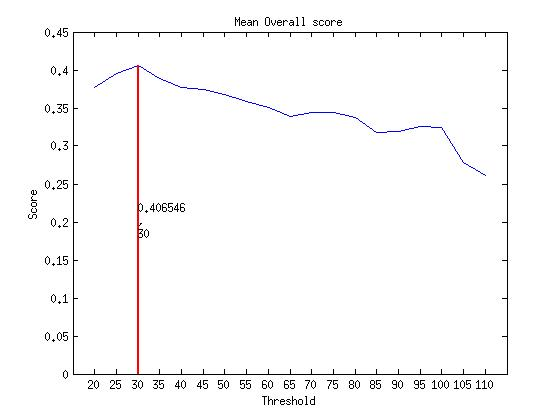
\includegraphics[scale=0.5]{../Drawings/OptimalParameters_SBRISK_SBRISK_KNN.jpg}
\caption{The optimal parameters for S-BRISK with KNN}
\label{fig:sbriskknnOptimal}
\end{minipage}
\hspace{0.5cm}
\begin{minipage}[b]{0.5\linewidth}
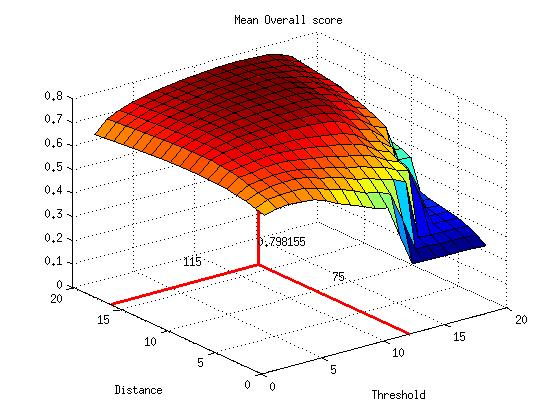
\includegraphics[scale=0.5]{../Drawings/OptimalParameters_SBRISK_SBRISK_hamming.jpg}
\caption{The optimal parameters for S-BRISK with Hamming Distance}
\label{fig:sbriskhammingOptimal}
\end{minipage}
\begin{minipage}[b]{0.5\linewidth}
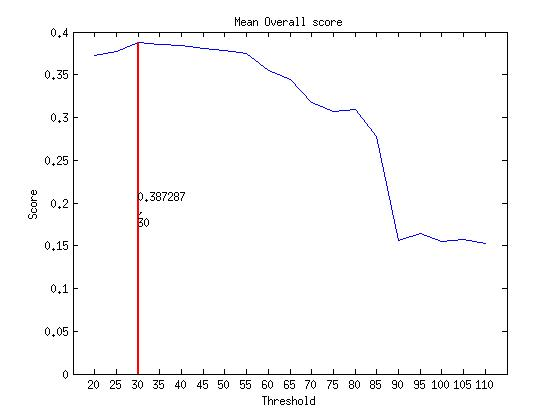
\includegraphics[scale=0.5]{../Drawings/OptimalParameters_BRISK4_BRISK4_KNN.jpg}
\caption{The optimal parameters for BRISK4 with KNN Distance}
\label{fig:brisk4knnOptimal}
\end{minipage}
\begin{minipage}[b]{0.5\linewidth}
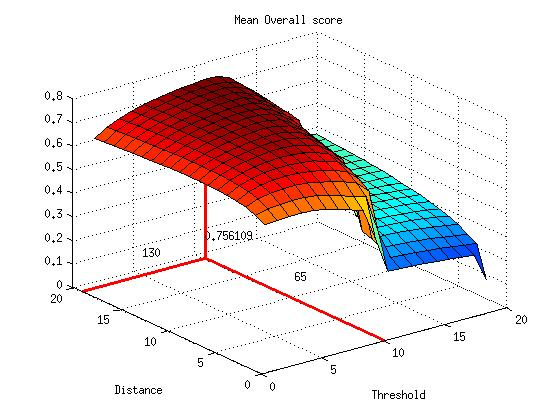
\includegraphics[scale=0.5]{../Drawings/OptimalParameters_BRISK4_BRISK4_Hamming.jpg}
\caption{The optimal parameters for BRISK4 with Hamming Distance}
\label{fig:brisk4hammingOptimal}
\end{minipage}
\begin{minipage}[b]{0.5\linewidth}
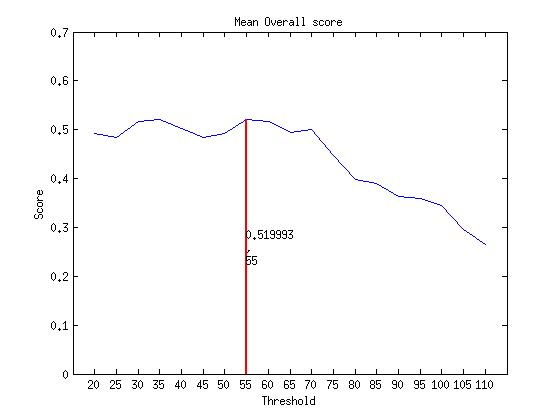
\includegraphics[scale=0.5]{../Drawings/OptimalParameters_SBRISK_SURF2D_KNN.jpg}
\caption{The optimal parameters for SBRISK SURF2D with KNN}
\label{fig:sbrisksurfknnOptimal}
\end{minipage}
\end{figure}

After performing the experiments a set of optimal parameters were generated. The parameter settings are shown in \tabref{tab:knnStatistics} and \tabref{tab:hammingStatistics} respectively. \textbf{TO ANALYSE}\\



\begin{table}
\caption{The optimal thresholds for the 2-KNN feature extraction algorithms}
\begin{tabular}{|c|c|c|c|c|c|c|c|c|}
\hline 
Detector & Extractor & Matcher & k1 & k2 & k3 & k4 & Normal threshold & Consistent threshold\tabularnewline
\hline 
\hline 
S-BRISK & S-BRISK & KNN=2 & 0.6 & 0.4 & 0.4 & 0.6 & 46.25 & 30\tabularnewline
\hline 
BRISK4 & BRISK4 & KNN=2 & 0.6 & 0.4 & 0.4 & 0.6 & 51.25 & 30\tabularnewline
\hline 
SBRISK & SURF2D & KNN=2 & 0.6 & 0.4 & 0.4 & 0.6 & 43.75 & 30\tabularnewline
\hline 
SBRISK & UBRISK & KNN=2 & 0.6 & 0.4 & 0.4 & 0.6 & 55 & 35\tabularnewline
\hline 
\end{tabular}
\label{tab:knnStatistics}
\end{table}

\begin{table}
\caption{The optimal thresholds for the Hamming/Euclidean distance feature extraction algorithms}
\begin{tabular}{|c|c|c|c|c|c|c|c|c|c|c|}
\hline 
Detector & Extractor & Matcher & k1 & k2 & k3 & k4 & thresholdM & distanceM & thresholdC & distanceC\tabularnewline
\hline 
\hline 
S-BRISK & S-BRISK & Hamming & 0.6 & 0.4 & 0.4 & 0.6 & 77.5 & 107.5 & 75 & 115\tabularnewline
\hline 
BRISK4 & BRISK4 & Hamming & 0.6 & 0.4 & 0.4 & 0.6 & 80 & 120 & 65 & 130\tabularnewline
\hline 
SBRISK & SURF2D & Euclidean & 0.6 & 0.4 & 0.4 & 0.6 & 65 & 0.28 & 60 & 0.28\tabularnewline
\hline 
SBRISK & UBRISK & Hamming & 0.6 & 0.4 & 0.4 & 0.6 & 75 & 121.25 & 75 & 130\tabularnewline
\hline 
\end{tabular}
\label{tab:hammingStatistics}
\end{table}

\subsubsection{Matching Score}
\label{sec:matchingScore}
As mentioned in \secref{sec:matching}, in the case of 2D SURF, keypoint pairs can be matched based on the euclidean distance between the feature vectors representing the keypoints. Similarly, in the case of BRISK, keypoints can be matched based on the hamming distance between the feature vectors. In both cases, taking the inverse distance can produce a matching score as shown in \eqnref{eqn:inverseDistance}. The smaller the distance between feature vectors, the more similar the keypoints become resulting in a high matching score and vice versa. In order to determine whether or not this score is a good metric for classifying whether images match or not, a number of tests were performed.

\begin{equation}
Score = \frac{1}{distance}
\label{eqn:inverseDistance}
\end{equation}

Utilising the images from the datasets in \tabref{table:overlap}, matching scores were computed for pairs of overlapping images and pairs of non-overlapping images respectively. It was expected that the matching score for the overlapping images would be larger than that of the non-overlapping images. \\

The feature extraction algorithms were utilised on all possible combinations of overlapping and non-overlapping image pairs respectively from each of the datasets. The algorithms include SBRISK, BRISK4, SBRISK-SURF2D and SBRISK- UBRISK. The matching criteria utilised was either K-Nearest Neighbors (KNN), Euclidean distance or Hamming distance depending on the method. The mean matching scores for $1421$ overlapping images and $2808$ non-overlapping images are shown in \tabref{tab:matchingScoreCompare}. \\

As can be seen in the table, matching scores for overlapping images are at least an order of magnitude larger than matching scores for non-overlapping images. This indicates that \eqnref{eqn:inverseDistance} can be utilised as a means to classify whether or not a match has occured between a pair of images. This score has been used to determine the overall performance of the feature extraction algorithms detailed in \secref{sec:overallPerformance}.\\

\begin{table}
\begin{tabular}{|c|c|c|}
\hline 
Method & Overlapping Score & Non-overlapping Score\tabularnewline
\hline 
\hline 
 & \multicolumn{2}{c}{2-KNN}\tabularnewline
\hline 
SBRISK & 0.213 & 0.002\tabularnewline
\hline 
BRISK4 & 0.167 & 0.002\tabularnewline
\hline 
SBRISK- SURF2D & 66.62 & 3.52\tabularnewline
\hline 
UBRISK & 0.177 & 0.001\tabularnewline
\hline 
 & \multicolumn{2}{c}{Hamming/Euclidean Distance}\tabularnewline
\hline 
SBRISK & 0.22 & 0.02\tabularnewline
\hline 
BRISK4 & 0.21 & 0.01\tabularnewline
\hline 
SBRISK- SURF2D & 50.16 & 3.15\tabularnewline
\hline 
UBRISK & 0.20 & 0.01\tabularnewline
\hline 
\end{tabular}
\label{tab:matchingScoreCompare}
\end{table}

\subsubsection{KNN Matching Constraint}
\label{sec:knnMatchingConstraint}
In order to verify the KNN matching constraint and determine the optimum threhsold, a number of tests were developed and implemented on the four main feature extraction techniques, namely SBRISK, BRISK4, UBRISK and SBRISK-2D SURF. In order to generate invalid matches, images with no overlap were compared and any matches found during the comparison were flagged as invalid matches. This was performed on $2808$ non-overlapping image pairs. To generate the valid matches, $108$ identical images were compared and all matches found between these images were flagged as valid matches. In both cases, 2-KNN matching was performed generating two matches for every keypoint. The ratio of the first and second KNN neighbor was then computed for both valid and invalid matches and the mean ratio was subsequently generated. The results are shown in \tabref{tab:knnCriterion} for each of the four methods. As can be seen in the table, invalid matches have a mean ratio which is over $0.9$. Valid matches have a ratio which is approximately zero. This illustrates a significant difference between the first and second KNN for valid and invalid matches. Based on this data, all matches whose KNN ratio is below $0.7$ are considered valid matches whereas all matches above $0.7$ are considered to be invalid matches. This value has been chosen in order to ensure that the majority of KNN invalid matches are rejected. Since the largest standard deviation is $8.8\%$ of the total KNN ratio value, a value well below $0.9$ has been selected. \\

In addition to this, the mean distance between the first and second KNN for each method have been computed. It has been found that there is a significant difference between the distances for valid and invalid matches respectively. The mean distance could also be used as a global threshold but this is not generic and some feature descriptors may be more discriminatory than others \cite{Lowe2004}. This is evident in the case of SBRISK-2D SURF as the standard deviation is $68\%$ of the total value indicating a huge amount of fluctuation about the mean. Thus the KNN ratio is a more useful constraint in this scenario.\\

\begin{table}
\caption{The KNN Ratios}
\begin{tabular}{|c|c|c|c|c|c|}
\hline 
Method & Match Type & Mean KNN Ratio & Std Deviation & Mean Distance between KNN neighbors & Std Deviation\tabularnewline
\hline 
\hline 
SBRISK & Invalid Matches & 0.94 & 0.06 & 7.45 & 7.58\tabularnewline
\hline 
 & Valid Matches & 0 & 0 & 97.66 & 37.97\tabularnewline
\hline 
BRISK4 & Invalid Matches & 0.93 & 0.06 & 7.93 & 7.91\tabularnewline
\hline 
 & Valid Matches & 0 & 0 & 86.47 & 42.78\tabularnewline
\hline 
SBRISK - UBRISK & Invalid Matches & 0.94 & 0.05 & 7.78 & 7.58\tabularnewline
\hline 
 & Valid Matches & 0 & 0 & 100.70 & 40.21\tabularnewline
\hline 
SBRISK SURF2D & Invalid Matches & 0.90 & 0.08 & 0.03 & 0.03\tabularnewline
\hline 
 & Valid Matches & 0.0004 & 0.0008 & 0.25 & 0.18\tabularnewline
\hline 
SURF 1D & Invalid Matches &  &  &  & \tabularnewline
\hline 
 & Valid Matches &  &  &  & \tabularnewline
\hline 
\end{tabular}
\label{tab:knnCriterion}
\end{table}


\subsubsection{Keypoint Matching Properties}
\label{sec:keypointMatching}
It is also important to determine whether or not keypoints corresponding to a valid match have different properties compared to keypoints corresponding to an invalid match. This could be useful in generating new constraints that can effectively remove invalid matches. Three criteria were analysed, namely the angle, size and response of each matched keypoint. In order to generate the useful statistics for this experiment, the angle, size and response of each of the keypoints in image $1$ are subtracted from the angle, size and response of the corresponding matched keypoints in image $2$. All of these differences are then summed together for all the matched keypoints each pair of images. The mean is subsequently computed. \\

The angle and response differences as well as the standard deviation for each of these differences are calculated using $40$ overlapping image pairs from all four datasets.\\
%The mean distance between 
In order to determine whether or not matches in images are valid, the two matching constraints discussed in \secref{sec:validation} have been utilised, namely, the angle and distance constraint and the the KNN ratio constraint. Utilising these constraints, overlapping image pairs were compared using the four feature extraction algorithms. The optimal \textit{maximum} parameter values from \tabref{tab:knnStatistics} have been used to perform these experiements. \\

The keypoints corresponding to valid and invalid matches in each of the images respectively were tabulated. Invalid matches due to the angle and distance constraints are tabulated separately from the invalid matches due to the KNN ratio constraint. The mean angle, response and size differences from the image pairs as well as the corresponding standard deviations are shown in \tabref{tab:keypointProperties}.\\

One of the more significant observations is the mean response difference. Valid matches from overlapping image pairs in all of the feature extraction algorithms have a mean response that is 

%The keypoints in image A were subtracted from the keypoints in image B.

\begin{table}
\caption{The properties of valid and invalid interest point matches}
\begin{tabular}{|c|c|c|c|c|c|r@{\extracolsep{0pt}.}l|}
\hline 
Property & \multicolumn{7}{c}{Invalid Matches due to Angle Constraint}\tabularnewline
\hline 
\hline 
Method & Mean Angle & Angle Std & Response & Response Std & Size & \multicolumn{2}{c|}{Size Std}\tabularnewline
\hline 
SBRISK & 20.28 & 6.680 & 0.5400 & 1.070 & 0 & \multicolumn{2}{c|}{0}\tabularnewline
\hline 
BRISK4 & 6.98 & 1.47 & 6.31 & 2.88 & 0.300 & 2&54\tabularnewline
\hline 
SBRISK - SURF2D & 0 & 0 & 0.4300 & 0.8900 & 0 & \multicolumn{2}{c|}{0}\tabularnewline
\hline 
UBRISK & 0 & 0 & 0.13 & 2.060 & 0 & \multicolumn{2}{c|}{0}\tabularnewline
\hline 
 & \multicolumn{7}{c}{Invalid Matches due to KNN Ratio Constraint}\tabularnewline
\hline 
SBRISK & 4.280 & 0.8700 & 6.810 & 1.980 & 0 & \multicolumn{2}{c|}{0}\tabularnewline
\hline 
BRISK4 & 3.24 & 4.84 & 2.43 & 1.03 & 3.02 & 4&58\tabularnewline
\hline 
SBRISK - SURF2D & 0 & 0 & 2.370 & 1.700 & 0 & \multicolumn{2}{c|}{0}\tabularnewline
\hline 
UBRISK & 0 & 0 & 4.610 & 1.710 & 0 & \multicolumn{2}{c|}{0}\tabularnewline
\hline 
 & \multicolumn{7}{c}{Valid Matches}\tabularnewline
\hline 
SBRISK & 0.6600 & 0.5200 & 0.08000 & 0.1000 & 0 & \multicolumn{2}{c|}{0}\tabularnewline
\hline 
BRISK4 & 1.20 & 0.310 & -0.860 & 0.0500 & -0.0900 & 0&410\tabularnewline
\hline 
SBRISK - SURF2D & 0 & 0 & 0.2900 & 0.2700 & 0 & \multicolumn{2}{c|}{0}\tabularnewline
\hline 
UBRISK & 0 & 0 & -0.11 & -0.44 & 0 & \multicolumn{2}{c|}{0}\tabularnewline
\hline 
\end{tabular}
\label{tab:keypointProperties}
\end{table}

%A picture of the graph for each method containing the optimal parameters


\subsection{Overall Performance}
\label{sec:overallPerformance}

%These tables will be needed when describing why some methods perform better than others. This will therefore be included in the overall performance section

%This data was generated by considering overlapping and non-overlapping images
%The valid matches and invalid matches should differ between the matching and overlapping sets respectively.

\begin{table}
\begin{tabular}{|c|c|c|c|c|}
\hline 
Method & \multicolumn{4}{c}{Overlapping images}\tabularnewline
\hline 
\hline 
 & Total Matches & Valid Matches & Invalid Matches & Mean Num Keypoints\tabularnewline
\hline 
SBRISK - 2KNN & 175.560 & 15.42 & 160.14 & 77.43000\tabularnewline
\hline 
BRISK4 - 2KNN & 175.6300 & 13.23000 & 162.4100 & 73.70000\tabularnewline
\hline 
SBRISK-SURF2D - 2KNN & 218.8800 & 19.01000 & 199.8600 & 97.88000\tabularnewline
\hline 
SBRISK - UBRISK & 135.7600 & 16.14000 & 119.6200 & 59.38000\tabularnewline
\hline 
 & \multicolumn{4}{c}{Non-overlapping images}\tabularnewline
\hline 
 &  &  &  & \tabularnewline
\hline 
SBRISK - 2KNN & 72.260 & 0.25000 & 72.010 & 77.430\tabularnewline
\hline 
BRISK4 - 2KNN & 69.930 & 0.28000 & 69.640 & 73.700\tabularnewline
\hline 
SBRISK-SURF2D - 2KNN & 98.700 & 1.3900 & 97.310 & 97.880\tabularnewline
\hline 
SBRISK - UBRISK & 54.560 & 0.22000 & 54.340 & 59.380\tabularnewline
\hline 
\end{tabular}
\label{tab:keypointsMatchesKNN}
\end{table}

\begin{table}
\begin{tabular}{|c|c|c|c|c|}
\hline 
Method & Total Matches & Valid Matches & Invalid Matches & Mean Num Keypoints\tabularnewline
\hline 
\hline 
 & \multicolumn{4}{c}{Overlapping images}\tabularnewline
\hline 
SBRISK - Hamming & 70.770 & 39.980 & 30.790 & 32.420\tabularnewline
\hline 
BRISK4 - Hamming & 91.380 & 57.510 & 33.870 & 31.560\tabularnewline
\hline 
SBRISK-SURF2D - Euclidean & 19.530 & 12.050 & 7.4800 & 51.940\tabularnewline
\hline 
SBRISK - UBRISK & 40.120 & 26.930 & 13.190 & 33.530\tabularnewline
\hline 
 & \multicolumn{4}{c}{Non-overlapping images}\tabularnewline
\hline 
SBRISK - Hamming & 11.150 & 4.9600 & 6.1900 & 32.420\tabularnewline
\hline 
BRISK4 - Hamming & 5.6300 & 2.3900 & 3.2500 & 31.560\tabularnewline
\hline 
SBRISK-SURF2D - Euclidean & 2.6800 & 0.90000 & 1.7800 & 51.940\tabularnewline
\hline 
SBRISK - UBRISK & 3.9700 & 1.8500 & 2.1200 & 33.530\tabularnewline
\hline 
\end{tabular}
\label{tab:keypointsMatchesHamming}
\end{table}

\begin{figure}[h!]
\begin{minipage}[b]{0.5\linewidth}
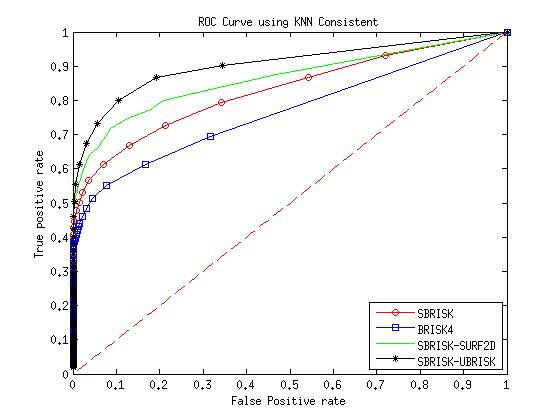
\includegraphics[scale=0.5]{../Drawings/ROC_General_Hamming.jpg}
\caption{A comparison of the ROC curves for SBRISK, BRISK4 and SBRISK-SURF2D using Hamming distance for matching}
\label{fig:compareHamming}
\end{minipage}
\hspace{0.5cm}
\begin{minipage}[b]{0.5\linewidth}
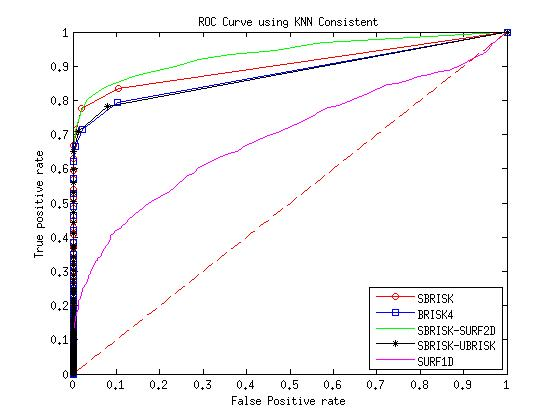
\includegraphics[scale=0.5]{../Drawings/ROC_General_KNN.jpg}
\caption{A comparison of the ROC curves for SBRISK, BRISK4 and SBRISK-SURF2D using 2-KNN for matching}
\label{fig:compareKNN}
\end{minipage}
\begin{minipage}[b]{0.5\linewidth}
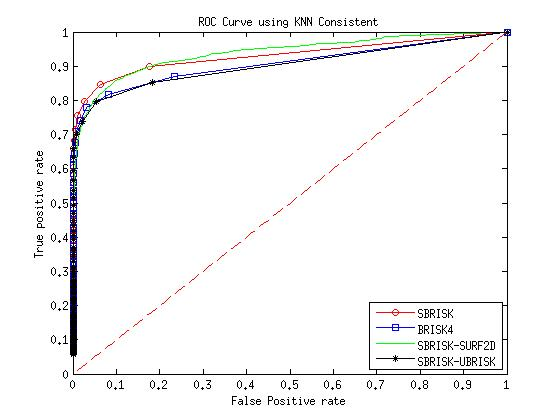
\includegraphics[scale=0.5]{../Drawings/ROC_General_KNN_Consistent.jpg}
\caption{A comparison of the ROC curves for SBRISK, BRISK4 and SBRISK-SURF2D using 2-KNN for matching and consistent thresholds}
\label{fig:compareKNNConsistent}
\end{minipage}
\end{figure}

\begin{table}
\caption{The performance statistics of 2-KNN feature extraction algorithms}
\begin{tabular}{|c|c|c|c|c|c|c|c|}
\hline 
\textbf{Method (2-KNN)} & Threshold & \% AUC & Detection(ms) & Extraction(ms) & Matching(ms) & Verification(ms) & Overall(ms)\tabularnewline
\hline 
\hline 
SBRISK & Maximum & 90.429 & 3.4840 & 6.0540 & 0.002 & 0.029 & 15.271\tabularnewline
\hline 
BRISK4 & Maximum & 88.084 & 10.882 & 5.8820 & 0.002 & 0.029 & 22.422\tabularnewline
\hline 
SBRISK - SURF2D & Maximum & 93.586 & 3.6230 & 12.016 & 0.001 & 0.039 & 20.304\tabularnewline
\hline 
SBRISK - U-BRISK & Maximum & 87.830 & 3.3320 & 2.5950 & 0.001 & 0.024 & 11.005\tabularnewline
\hline 
SBRISK & Consistent & 93.064 & 4.1300 & 11.108 & 0.006 & 0.053 & 25.810\tabularnewline
\hline 
BRISK4 & Consistent & 90.768 & 15.842 & 10.970 & 0.007 & 0.057 & 37.662\tabularnewline
\hline 
SBRISK - SURF2D & Consistent & 93.799 & 4.2050 & 20.799 & 0.001 & 0.067 & 30.628\tabularnewline
\hline 
SBRISK - U-BRISK & Consistent & 90.350 & 3.8320 & 4.0510 & 0.004 & 0.042 & 15.709\tabularnewline
\hline 
\end{tabular}
\label{tab:keypointsMatchesHamming}
\end{table}

\begin{table}
\caption{The performance statistics of Hamming/Euclidean Distance feature extraction algorithms}
\begin{tabular}{|c|c|c|c|c|c|c|c|}
\hline 
Method & Threshold, distance & \% AUC & Detection(ms) & Extraction(ms) & Matching(ms) & Verification(ms) & Overall(ms)\tabularnewline
\hline 
\hline 
SBRISK & Maximum & 82.908 & 3.080 & 3.218 & 0 & 0.01600 & 10.717\tabularnewline
\hline 
BRISK4 & Maximum & 76.616 & 8.492 & 3.355 & 0 & 0.01600 & 16.259\tabularnewline
\hline 
SBRISK-SURF2D & Maximum & 86.347 & 3.231 & 7.299 & 0 & 0.009000 & 14.865\tabularnewline
\hline 
SBRISK-UBRISK & Maximum & 90.378 & 3.097 & 1.953 & 0 & 0.01000 & 9.431\tabularnewline
\hline 
\end{tabular}

\label{tab:hammingStatistics}
\end{table}





\subsubsection{SURF2D}
\label{sec:2dsurfResults}
%1. Picture of the ROC curve
%STATS:
%a. The AUC
%b. average time, extraction, deletion
%c. Performance under lighting, scale, rotation and image blur

\subsubsection{BRISK}
\label{sec:briskResults}
%Find the optimal parameters:
%1. threshold only + KNN
%\begin{table}
%\caption{Optimum Threshold}
%\begin{tabular}{|c|c|c|c|c|c|c|c|c|}
%\hline 
%Detector & Extractor & Matcher & k1 & k2 & k3 & k4 & threshold & thresholdC\tabularnewline
%\hline 
%\hline 
%BRISK4 & BRISK4 & KNN=2 & 0.6 & 0.4 & 0.4 & 0.6 & 51.25 & 30\tabularnewline
%\hline 
%\end{tabular}
%\label{tab:sbrisk}
%\end{table}

%\begin{figure}[h!]
%	\centering
%		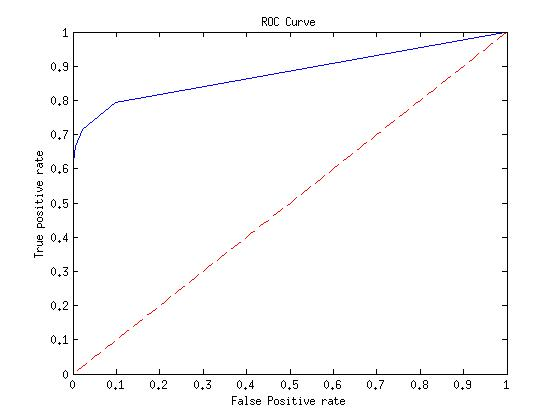
\includegraphics[width=0.6\textwidth]{../Drawings/ROC_BRISK4_BRISK4_KNN.jpg}
%	\caption{The ROC Curve for BRISK4 KNN}
%	\label{fig:sbriskroc}
%\end{figure}

%\begin{table}
%\caption{Optimum Threshold}
%\begin{tabular}{|c|c|c|c|c|c|c|c|c|}
%\hline 
%\% AUC & Detection(ms) & Extraction(ms) & Matching(ms) & Verification(ms) & Overall(ms) & OP & \% TP & \% FP\tabularnewline
%\hline 
%\hline 
%88.08 & 19.43 & 9.34 & 1.54 & 0.03 & 39.06 &  &  & \tabularnewline
%\hline 
%90.76 & 27.79 & 18.00 & 6.81 & 0.05 & 61.30 &  &  & \tabularnewline
%\hline 
%\end{tabular}
%\label{tab:sbrisk}
%\end{table}

%2. threshold, hammingdistance + KNN
%****************************************************************
%\begin{table}
%\caption{Optimum Threshold}
%\begin{tabular}{|c|c|c|c|c|c|c|c|c|c|c|}
%\hline 
%Detector & Extractor & Matcher & k1 & k2 & k3 & k4 & threshold & distance & thresholdC & distanceC\tabularnewline
%\hline 
%\hline 
%BRISK4 & BRISK4 & Hamming & 0.6 & 0.4 & 0.4 & 0.6 & 85 & 121.25 & 130 & 65\tabularnewline
%\hline 
%\end{tabular}
%\label{tab:sbrisk}
%\end{table}

%1. Picture of the ROC curve
%STATS:
%a. The AUC
%b. average time, extraction, deletion
%\begin{figure}[h!]
%	\centering
%		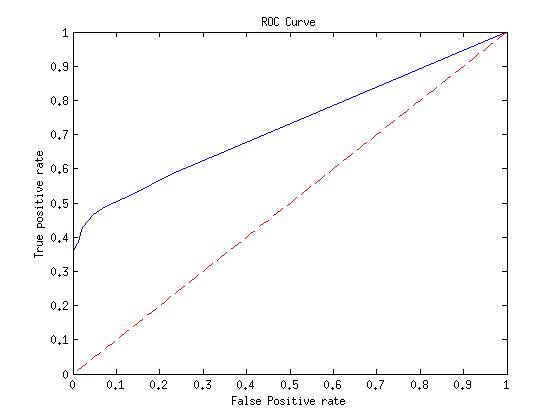
\includegraphics[width=0.6\textwidth]{../Drawings/ROC_BRISK4_BRISK4_Hamming.jpg}
%	\caption{The ROC Curve for BRISK4 Hamming}
%	\label{fig:sbriskroc}
%\end{figure}

%\begin{table}
%\caption{Optimum Threshold}
%\begin{tabular}{|c|c|c|c|c|c|c|c|c|}
%\hline 
%\% AUC & Detection(ms) & Extraction(ms) & Matching(ms) & Verification(ms) & Overall(ms) & OP & \% TP & \% FP\tabularnewline
%\hline 
%\hline 
%74.36 & 14.55 & 4.42 & 0.26 & 0.01 & 27.87 &  &  & \tabularnewline
%\hline 
%\end{tabular}
%\end{table}


\subsubsection{BRISK-SURF2D}
\label{sec:brisk2dsurfResults}
%1. Picture of the ROC curve

%\begin{table}
%\caption{Optimum Threshold}
%\begin{tabular}{|c|c|c|c|c|c|c|c|c|}
%\hline 
%Detector & Extractor & Matcher & k1 & k2 & k3 & k4 & threshold & thresholdC\tabularnewline
%\hline 
%\hline 
%SBRISK & SURF2D & KNN=2 & 0.6 & 0.4 & 0.4 & 0.6 & 45 & 35\tabularnewline
%\hline 
%\end{tabular}
%\label{tab:sbrisk}
%\end{table}

%\begin{figure}[h!]
%	\centering
%		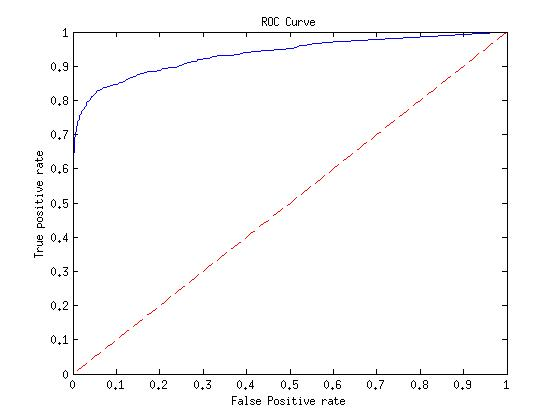
\includegraphics[width=0.6\textwidth]{../Drawings/ROC_SBRISK_SURF2D_KNN.jpg}
%	\caption{The ROC Curve for SBRISK SURF2D KNN}
%	\label{fig:sbriskroc}
%\end{figure}


%\begin{table}
%\caption{Optimum Threshold}
%\begin{tabular}{|c|c|c|c|c|c|c|c|c|}
%\hline 
%\% AUC & Detection(ms) & Extraction(ms) & Matching(ms) & Verification(ms) & Overall(ms) & OP & \% TP & \% FP\tabularnewline
%\hline 
%\hline 
%93.53 & 6.07 & 17.99 & 0.54 & 0.03 & 33.26 &  &  & \tabularnewline
%\hline 
%93.79 & 7.00 & 32.86 & 1.45 & 0.06 & 49.78 &  &  & \tabularnewline
%\hline 
%\end{tabular}
%\end{table}
%STATS:
%a. The AUC
%b. average time, extraction, deletion
%\begin{figure}[h!]
%	\centering
%		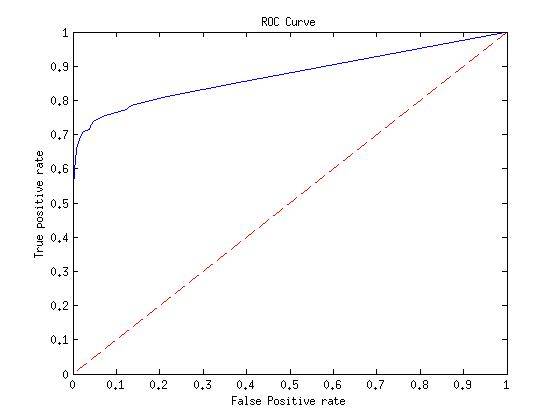
\includegraphics[width=0.6\textwidth]{../Drawings/ROC_SBRISK_SURF2D_Hamming.jpg}
%	\caption{The ROC Curve for SBRISK SURF2D Hamming}
%	\label{fig:sbriskroc}
%\end{figure}


%2. threshold, hammingdistance + KNN
%****************************************************************
%\begin{table}
%\caption{Optimum Threshold}
%\begin{tabular}{|c|c|c|c|c|c|c|c|c|c|c|}
%\hline 
%Detector & Extractor & Matcher & k1 & k2 & k3 & k4 & threshold & distance & thresholdC & distanceC\tabularnewline
%\hline 
%\hline 
%SBRISK & SURF2D & Hamming & 0.6 & 0.4 & 0.4 & 0.6 & 65 & 0.28 & 60 & 0.28\tabularnewline
%\hline 
%\end{tabular}
%\label{tab:sbrisk}
%\end{table}


%\begin{table}
%\caption{Optimum Threshold}
%\begin{tabular}{|c|c|c|c|c|c|c|c|c|}
%\hline 
%\% AUC & Detection(ms) & Extraction(ms) & Matching(ms) & Verification(ms) & Overall(ms) & OP & \% TP & \% FP\tabularnewline
%\hline 
%\hline 
%87.37 & 16.7 & 87.19 & 0.43 & 0.01 & 112.97 &  &  & \tabularnewline
%\hline 
%\end{tabular}
%\label{tab:sbrisk}
%\end{table}


%STATS:
%a. The AUC
%b. average time, extraction, deletion


\subsubsection{S-BRISK}
\label{sec:sbriskResults}
%Find the optimal parameters:
%1. threshold only + KNN
%\begin{table}
%\caption{Optimum Threshold}
%\begin{tabular}{|c|c|c|c|c|c|c|c|c|}
%\hline 
%Detector & Extractor & Matcher & k1 & k2 & k3 & k4 & threshold & thresholdC\tabularnewline
%\hline 
%\hline 
%S-BRISK & S-BRISK & KNN=2 & 0.6 & 0.4 & 0.4 & 0.6 & 46.25 & 30\tabularnewline
%\hline 
%\end{tabular}
%\label{tab:sbrisk}
%\end{table}

%1. Picture of the ROC curve
%STATS:
%a. The AUC
%b. average time, extraction, deletion

%\begin{figure}[h!]
%	\centering
%		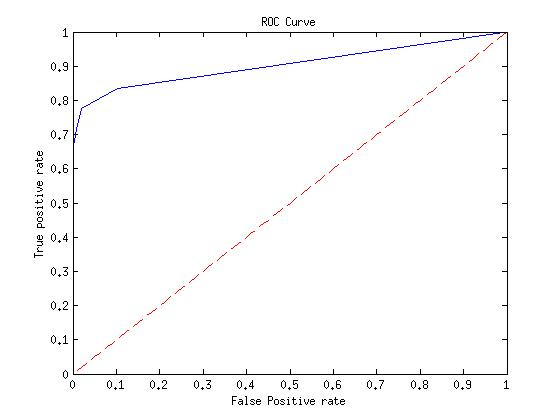
\includegraphics[width=0.6\textwidth]{../Drawings/ROC_SBRISK_SBRISK_KNN.jpg}
%	\caption{The ROC Curve for S-BRISK with KNN}
%	\label{fig:sbriskroc}
%\end{figure}

%\begin{table}
%\caption{Optimum Threshold}
%\begin{tabular}{|c|c|c|c|c|c|c|c|c|}
%\hline 
%\% AUC & Detection(ms) & Extraction(ms) & Matching(ms) & Verification(ms) & Overall(ms) & OP & \% TP & \% FP\tabularnewline
%\hline 
%\hline 
%90.31 & 5.85 & 8.79 & 1.89 & 0.04 & 24.98 &  &  & \tabularnewline
%\hline 
%93.06 & 7.07 & 17.08 & 6.52 & 0.05 & 39.17 &  &  & \tabularnewline
%\hline 
%\end{tabular}
%\label{tab:sbrisk}
%\end{table}


%2. threshold, hammingdistance + KNN
%****************************************************************
%\begin{table}
%\caption{Optimum Threshold}
%\begin{tabular}{|c|c|c|c|c|c|c|c|c|c|c|}
%\hline 
%Detector & Extractor & Matcher & k1 & k2 & k3 & k4 & threshold & distance & thresholdC & distanceC\tabularnewline
%\hline 
%\hline 
%S-BRISK & S-BRISK & Hamming & 0.6 & 0.4 & 0.4 & 0.6 & 78.75 & 110 & 75 & 115\tabularnewline
%\hline 
%\end{tabular}
%\label{tab:sbrisk}
%\end{table}

%\begin{figure}[h!]
%	\centering
%		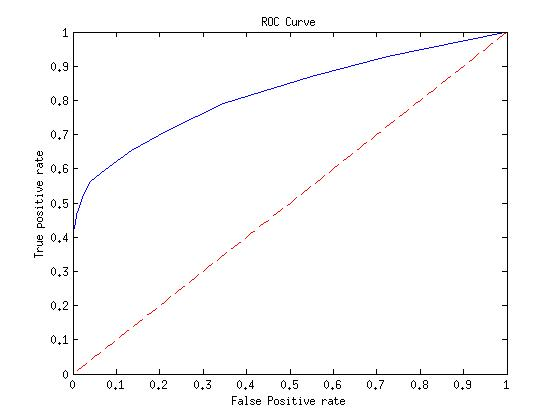
\includegraphics[width=0.6\textwidth]{../Drawings/ROC_SBRISK_SBRISK_Hamming.jpg}
%	\caption{The ROC Curve for S-BRISK using Hamming distance}
%	\label{fig:sbriskrocHamming}
%\end{figure}


%\begin{tabular}{|c|c|c|c|c|c|c|c|c|}
%\hline 
%\% AUC & Detection(ms) & Extraction(ms) & Matching(ms) & Verification(ms) & Overall(ms) & OP & \% TP & \% FP\tabularnewline
%\hline 
%\hline 
%82.24 & 5.15 & 4.62 & 0.33 & 0.01 & 18.63 &  &  & \tabularnewline
%\hline 
%\end{tabular}




%1. Picture of the ROC curve
%STATS:
%a. The AUC
%b. average time, extraction, deletion

\subsubsection{1DSURF}
\label{sec:1dsurfResults}
%1. Picture of the ROC curve
%STATS:
%a. The AUC
%b. average time, extraction, deletion


\subsection{Localisation Performance}
\label{sec:localisationPerformance}







\section{Conclusion}
\label{sec:conclusion}

\bibliographystyle{witseie}
\bibliography{bibliography}
% \newpage
%\onecolumn
%\appendix
%\setcounter{table}{0}
%\setcounter{figure}{0}
%\setcounter{subsection}{0}
%\makeatletter \renewcommand{\thefigure}{A.\@arabic\c@figure} \renewcommand{\thetable}{A.\@arabic\c@table} \renewcommand{\thesection}{A.\@arabic\c@section} \makeatother
%\section*{APPENDIX A}
%
%\section{Control Program}
%Add the matlab code to this file...
%\lstinputlisting{codeSnippets.cpp}
 
\end{document}

